\documentclass[10pt]{article}
\usepackage[margin=0.72in]{geometry}
\usepackage[T1]{fontenc}
\usepackage{lmodern,microtype,booktabs,graphicx,xcolor,hyperref,placeins}
\definecolor{navy}{HTML}{16324F}\definecolor{teal}{HTML}{087E8B}
\hypersetup{colorlinks=true,linkcolor=navy,urlcolor=teal}
\title{\textcolor{navy}{Does Cluster-Local Adaptation Transfer?}\\[3pt]
\large A Fresh-Seed Comparison Across Task Families and Drift Mechanisms}
\author{23I-2581 and 23I-2604\\Data Analysis and Visualization --- Phase 3 research addendum}
\date{18 November 2026}
\begin{document}\maketitle
\begin{abstract}
We broaden the matched-clock adaptation comparison beyond one linear abrupt-reversal example. Thirty fresh evaluation seeds cover three task families, four stream mechanisms and feedback delays 0, 5 and 20. Frozen, global-refit and cluster-local-refit models share update clocks and released row-ID windows. The comparison reveals strong task dependence: local models improve accuracy in the five-region and XOR generators, including stationary streams, but slightly underperform global refitting in most linear settings. The stationary gains show that this design does not isolate a drift-specific benefit of local adaptation.
\end{abstract}
\section{Protocol}
Each stream contains 96 batches of 500 rows, with 4,000 initial training rows. A training-fitted scaler and three-cluster MiniBatchKMeans assignment remain frozen. The two adaptive arms receive the same latest released feedback IDs at clocks 25, 49, 73 and 89; each refit uses at most 2,000 rows and repeated row uses count toward an 8,000-row cap. The local arm fits separate logistic models by frozen cluster and falls back to the initial global model when a cluster has fewer than 20 rows or only one observed class. Both arms receive the same opportunity schedule and feedback window, but they do not have equal parameter counts or equal CPU cost. Source labels obey $s+d<b$ for a prediction at batch $b$.

The task families are linear probabilistic classification, XOR classification and a five-region generator. The mechanisms are stationary, gradual predictive-feature shift, recurrent conditional reversal and out-of-support displacement. The 30-seed evaluation bank (73116301--73116330) was checked against existing text manifests and archive metadata; no exact collisions were found. Within each seed, comparisons are paired across task, mechanism and delay. The run is a broad sensitivity extension, not a newly tuned primary analysis; the 95\% intervals shown are per-setting and unadjusted across the 36 local--global comparisons.
\section{Results}
\begin{figure}[ht]
\centering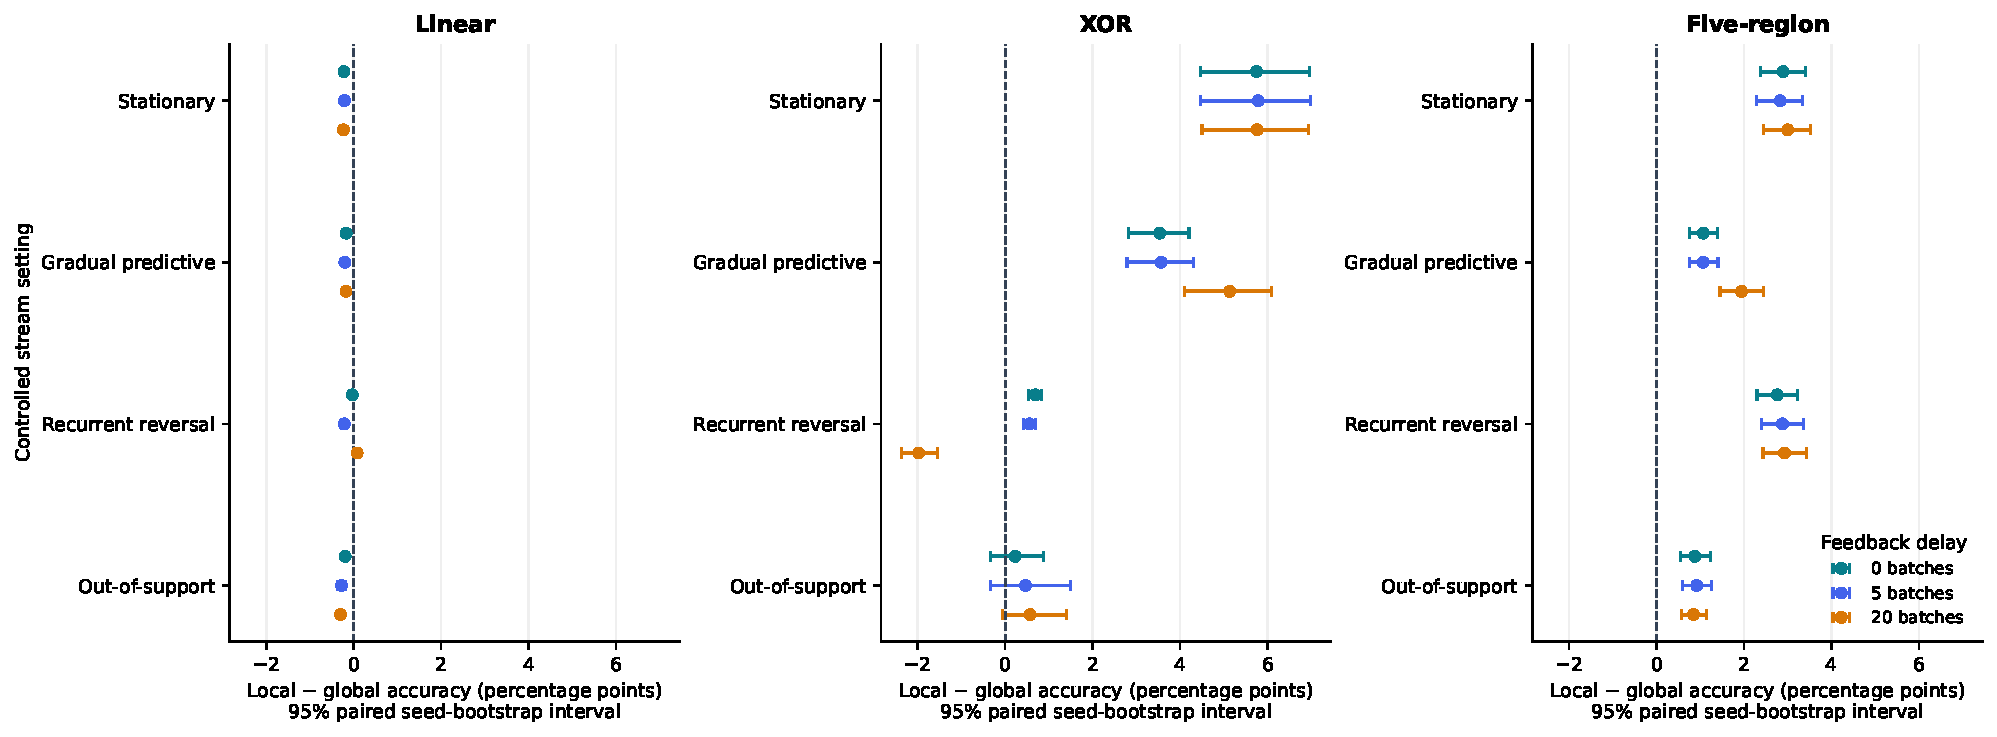
\includegraphics[width=\linewidth]{adaptation_diversity_effects.pdf}
\caption{Cluster-local minus global-refit all-stream accuracy, in percentage points. Points and intervals are paired across the same 30 seeds. Intervals are descriptive and unadjusted for the 36 settings. Positive values favor the local arm in this specific design.}
\end{figure}
\begin{table}[ht]
\centering\small\begin{tabular}{@{}llrrrr@{}}\toprule
Task & Mechanism & Frozen & Global & Local & Local--global (pp)\\\midrule
Linear & Stationary & 0.725 & 0.724 & 0.722 & -0.22 \\
Linear & Gradual predictive & 0.757 & 0.757 & 0.755 & -0.18 \\
Linear & Recurrent reversal & 0.575 & 0.550 & 0.549 & -0.06 \\
Linear & Out-of-support & 0.731 & 0.731 & 0.728 & -0.26 \\
XOR & Stationary & 0.578 & 0.577 & 0.634 & +5.77 \\
XOR & Gradual predictive & 0.551 & 0.656 & 0.697 & +4.08 \\
XOR & Recurrent reversal & 0.527 & 0.517 & 0.514 & -0.24 \\
XOR & Out-of-support & 0.810 & 0.803 & 0.808 & +0.42 \\
Five-region & Stationary & 0.524 & 0.525 & 0.554 & +2.91 \\
Five-region & Gradual predictive & 0.527 & 0.579 & 0.592 & +1.36 \\
Five-region & Recurrent reversal & 0.518 & 0.515 & 0.544 & +2.86 \\
Five-region & Out-of-support & 0.581 & 0.647 & 0.656 & +0.88 \\\bottomrule\end{tabular}
\caption{Accuracy averages first over the three delays and then over the 30 seeds. Local--global values average the paired setting-level differences over delays.}\end{table}
\FloatBarrier
\section{Interpretation}
The local--global effect changes sign across task families. For the five-region task, the local arm is higher in all four mechanisms, with delay-averaged differences ranging from roughly 0.88 to 2.91 percentage points. The XOR task shows larger local gains under stationarity and gradual shift, but the recurrent-reversal effect is small and becomes negative at delay 20; out-of-support differences are small and their intervals include zero. In the linear task, local refitting is generally slightly worse, although the recurrent-reversal comparison at delay 20 is a small positive exception. At the same time, local-vs-frozen post-onset accuracy in stationary data rises by about 3.96 points for the five-region task and 7.49 points for XOR, while it falls by about 0.40 points for the linear task. Therefore, improvements in regional and XOR cases can arise from the cluster-gated model's greater representational capacity, not solely from adaptation to drift. This is an important comparator limitation and a reason not to claim local adaptation is generally superior.

Global refitting also does not guarantee improvement: under recurrent reversal in the linear and XOR families, both adaptive arms underperform their frozen comparators on average. Out-of-support shifts benefit the five-region arm but not the linear or XOR arms. These heterogeneous effects argue against collapsing mechanisms or task families into one overall ranking.
\section{Limitations}
This experiment holds update clocks and label windows fixed; it does not compare the trigger policy's value of choosing when to adapt. It uses a single logistic family, one three-cluster partition and simulated labels. The global and local arms have different effective model capacities and the local arm can consume fewer fitting rows when fallbacks occur (549 unsupported local-cluster fits across the evaluated cells). No natural-stream adaptation is included. Wall time is recorded, but memory, energy and acquisition prices are not measured. The seed bootstrap supports within-generator variability only; it does not make task generators equivalent to independent real-world datasets. No human decision-effect or causal claim is made.
\section{Reproduction}
From the workspace root:
\begin{verbatim}
powershell -ExecutionPolicy Bypass -File scripts/reproduce_adaptation_diversity.ps1
\end{verbatim}
The reproduction script creates new timestamped output paths and uses the same locked configuration. The run receipt includes source/config/output hashes, environment versions, seeds, timing and the exact matrix. The accompanying contract tests check cell counts, timing, matched IDs, row-use limits and report hashes.
\end{document}
